\documentclass{standalone}
\usepackage{tikz}
\usetikzlibrary{patterns, positioning}
\usetikzlibrary{shapes.misc}
\usepackage[outline]{contour}
\contourlength{1.5pt} 
\usepackage[sfdefault]{ClearSans} %% option 'sfdefault' activates Clear Sans as the default text font
\usepackage[T1]{fontenc}

\begin{document}
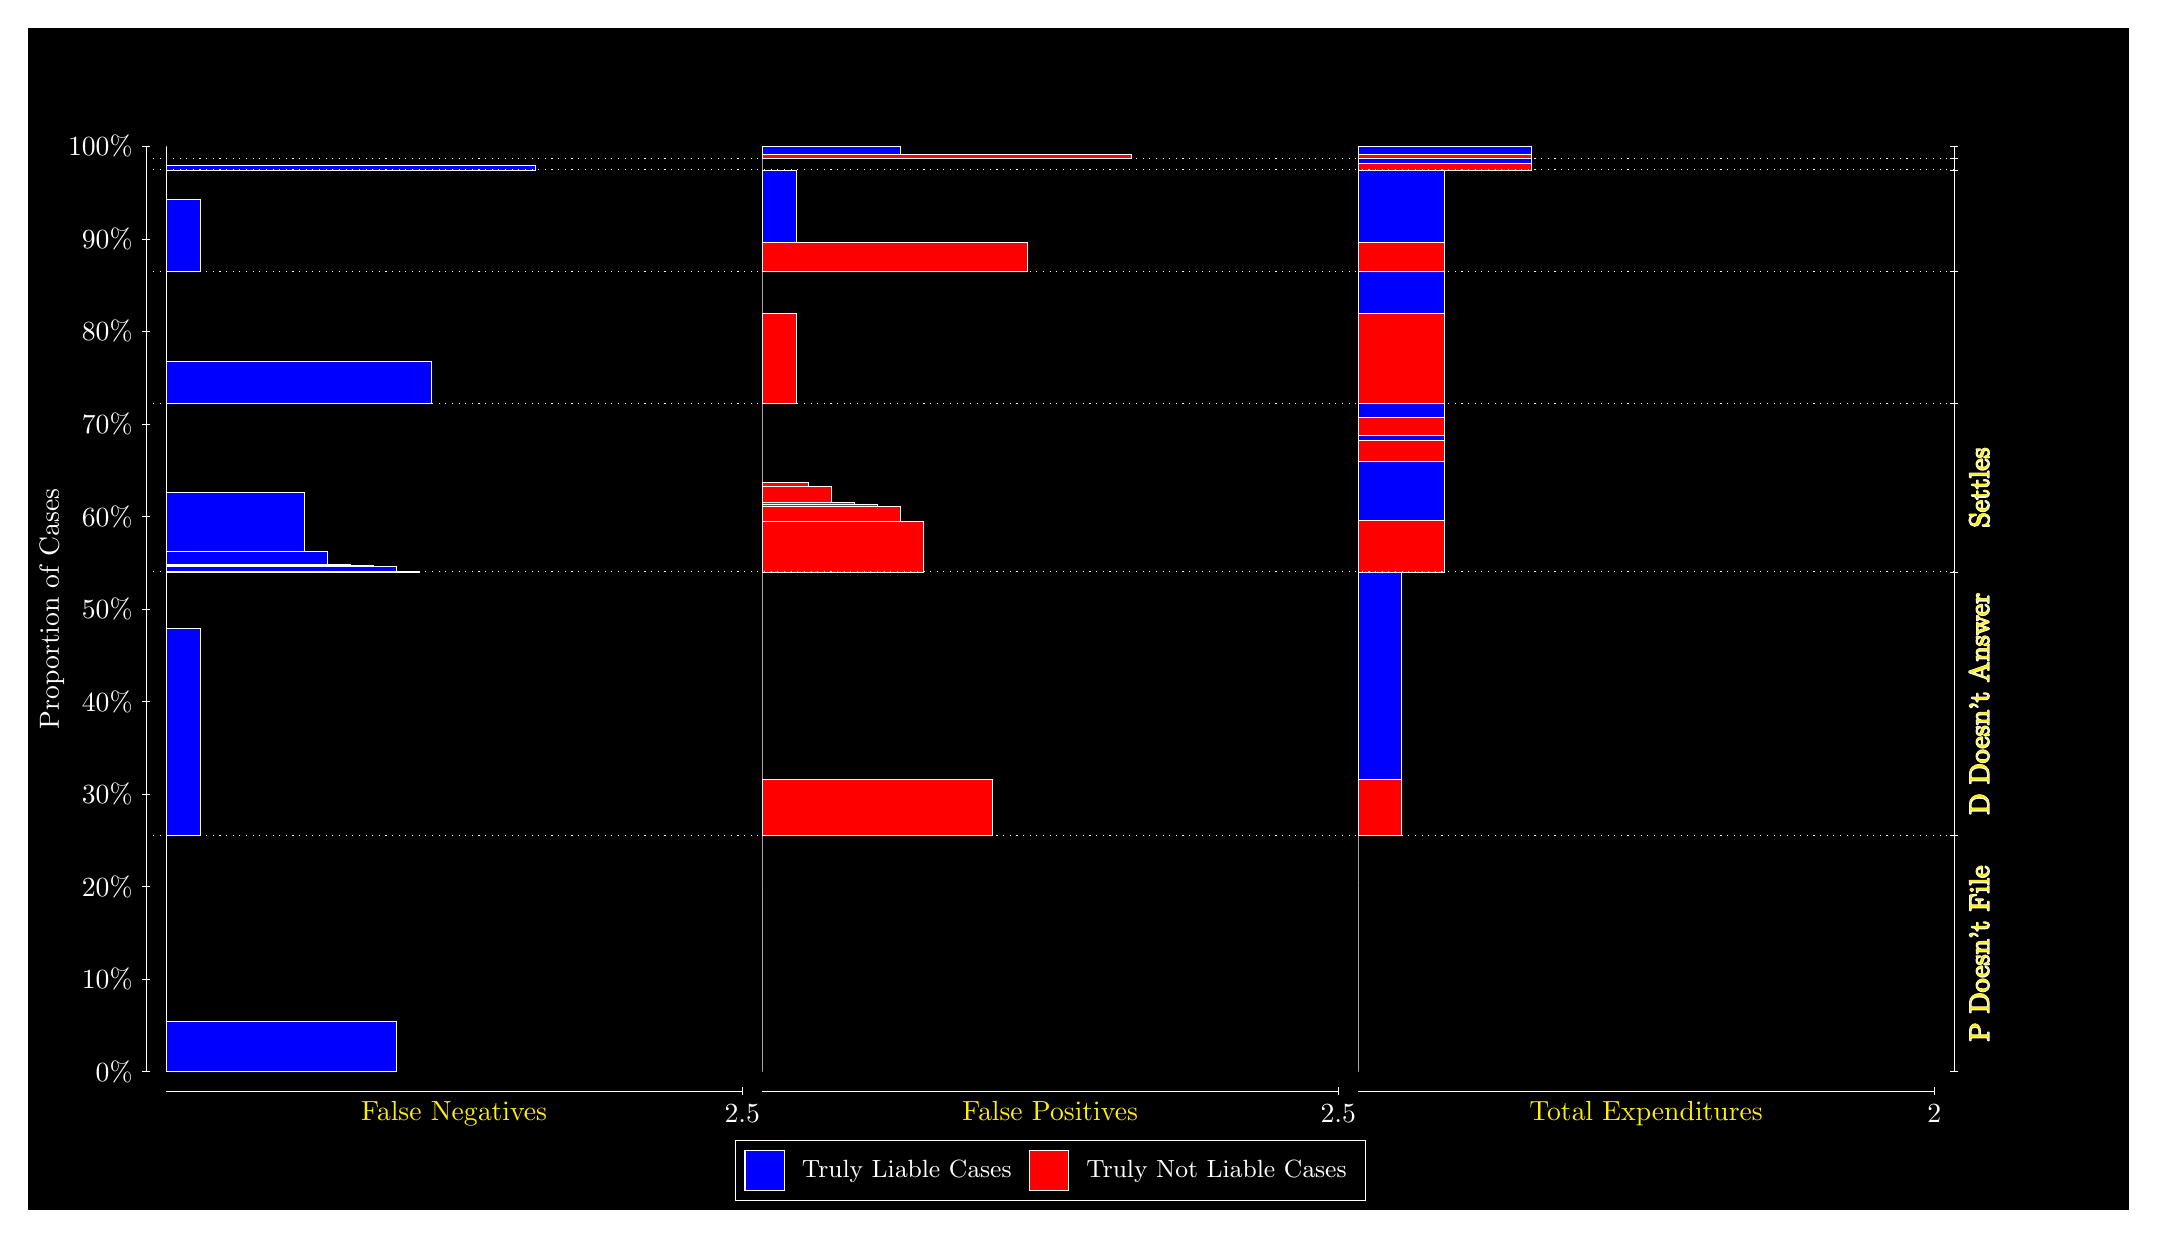
\begin{tikzpicture}
\draw[fill=black] (0,0) rectangle (26.667,15);
\draw[white, very thin] (1.5,1.75) -- (1.5,13.5);
\node[rotate=90, text=white, anchor=center] at (0.3, 7.625) {Proportion of Cases};
\draw[white, very thin] (1.45,1.75) -- (1.55,1.75);
\node[text=white, anchor=east] at (1.45, 1.75) {0\%};
\draw[white, very thin] (1.45,2.925) -- (1.55,2.925);
\node[text=white, anchor=east] at (1.45, 2.925) {10\%};
\draw[white, very thin] (1.45,4.1) -- (1.55,4.1);
\node[text=white, anchor=east] at (1.45, 4.1) {20\%};
\draw[white, very thin] (1.45,5.275) -- (1.55,5.275);
\node[text=white, anchor=east] at (1.45, 5.275) {30\%};
\draw[white, very thin] (1.45,6.45) -- (1.55,6.45);
\node[text=white, anchor=east] at (1.45, 6.45) {40\%};
\draw[white, very thin] (1.45,7.625) -- (1.55,7.625);
\node[text=white, anchor=east] at (1.45, 7.625) {50\%};
\draw[white, very thin] (1.45,8.8) -- (1.55,8.8);
\node[text=white, anchor=east] at (1.45, 8.8) {60\%};
\draw[white, very thin] (1.45,9.975) -- (1.55,9.975);
\node[text=white, anchor=east] at (1.45, 9.975) {70\%};
\draw[white, very thin] (1.45,11.15) -- (1.55,11.15);
\node[text=white, anchor=east] at (1.45, 11.15) {80\%};
\draw[white, very thin] (1.45,12.325) -- (1.55,12.325);
\node[text=white, anchor=east] at (1.45, 12.325) {90\%};
\draw[white, very thin] (1.45,13.5) -- (1.55,13.5);
\node[text=white, anchor=east] at (1.45, 13.5) {100\%};

\draw[white, very thin] (24.457,1.75) -- (24.457,13.5);
\draw[white, very thin] (24.407,1.75) -- (24.507,1.75);
\node[anchor=west] at (24.407, 1.75) {};
\draw[white, very thin] (24.407,4.7459) -- (24.507,4.7459);
\node[anchor=west] at (24.407, 4.7459) {};
\draw[white, very thin] (24.407,8.0951) -- (24.507,8.0951);
\node[anchor=west] at (24.407, 8.0951) {};
\draw[white, very thin] (24.407,10.239) -- (24.507,10.239);
\node[anchor=west] at (24.407, 10.239) {};
\draw[white, very thin] (24.407,11.909) -- (24.507,11.909);
\node[anchor=west] at (24.407, 11.909) {};
\draw[white, very thin] (24.407,13.2) -- (24.507,13.2);
\node[anchor=west] at (24.407, 13.2) {};
\draw[white, very thin] (24.407,13.342) -- (24.507,13.342);
\node[anchor=west] at (24.407, 13.342) {};
\draw[white, very thin] (24.407,13.5) -- (24.507,13.5);
\node[anchor=west] at (24.407, 13.5) {};

\draw[white, very thin, fill=blue] (1.75,1.75) rectangle (4.6775,2.3859);
\draw[white, very thin, fill=red] (1.75,2.3859) rectangle (1.75,4.7459);
\draw[white, very thin, fill=blue] (1.75,4.7459) rectangle (2.1891,7.3825);
\draw[white, very thin, fill=red] (1.75,7.3825) rectangle (1.75,8.0951);
\draw[white, very thin, fill=blue] (1.75,8.0951) rectangle (4.9703,8.1065);
\draw[white, very thin, fill=blue] (1.75,8.1065) rectangle (4.6775,8.1646);
\draw[white, very thin, fill=blue] (1.75,8.1646) rectangle (4.3848,8.1737);
\draw[white, very thin, fill=blue] (1.75,8.1737) rectangle (4.092,8.1942);
\draw[white, very thin, fill=blue] (1.75,8.1942) rectangle (3.7993,8.3587);
\draw[white, very thin, fill=blue] (1.75,8.3587) rectangle (3.5065,9.1028);
\draw[white, very thin, fill=red] (1.75,9.1028) rectangle (1.75,10.239);
\draw[white, very thin, fill=blue] (1.75,10.239) rectangle (5.1167,10.765);
\draw[white, very thin, fill=red] (1.75,10.765) rectangle (1.75,11.909);
\draw[white, very thin, fill=blue] (1.75,11.909) rectangle (2.1891,12.823);
\draw[white, very thin, fill=red] (1.75,12.823) rectangle (1.75,13.2);
\draw[white, very thin, fill=blue] (1.75,13.2) rectangle (6.4341,13.26);
\draw[white, very thin, fill=red] (1.75,13.26) rectangle (1.75,13.342);
\draw[white, very thin, fill=red] (1.75,13.342) rectangle (1.75,13.404);
\draw[white, very thin, fill=blue] (1.75,13.404) rectangle (1.75,13.5);
\draw[white, very thin, fill=red] (9.3189,1.75) rectangle (9.3189,4.11);
\draw[white, very thin, fill=blue] (9.3189,4.11) rectangle (9.3189,4.7459);
\draw[white, very thin, fill=red] (9.3189,4.7459) rectangle (12.246,5.4585);
\draw[white, very thin, fill=blue] (9.3189,5.4585) rectangle (9.3189,8.0951);
\draw[white, very thin, fill=red] (9.3189,8.0951) rectangle (11.368,8.7345);
\draw[white, very thin, fill=red] (9.3189,8.7345) rectangle (11.075,8.9296);
\draw[white, very thin, fill=red] (9.3189,8.9296) rectangle (10.783,8.9573);
\draw[white, very thin, fill=red] (9.3189,8.9573) rectangle (10.49,8.9755);
\draw[white, very thin, fill=red] (9.3189,8.9755) rectangle (10.197,9.1857);
\draw[white, very thin, fill=red] (9.3189,9.1857) rectangle (9.9044,9.2315);
\draw[white, very thin, fill=blue] (9.3189,9.2315) rectangle (9.3189,10.239);
\draw[white, very thin, fill=red] (9.3189,10.239) rectangle (9.758,11.383);
\draw[white, very thin, fill=blue] (9.3189,11.383) rectangle (9.3189,11.909);
\draw[white, very thin, fill=red] (9.3189,11.909) rectangle (12.686,12.287);
\draw[white, very thin, fill=blue] (9.3189,12.287) rectangle (9.758,13.2);
\draw[white, very thin, fill=red] (9.3189,13.2) rectangle (9.3189,13.282);
\draw[white, very thin, fill=blue] (9.3189,13.282) rectangle (9.3189,13.342);
\draw[white, very thin, fill=red] (9.3189,13.342) rectangle (14.003,13.404);
\draw[white, very thin, fill=blue] (9.3189,13.404) rectangle (11.075,13.5);
\draw[white, very thin, fill=red] (16.888,1.75) rectangle (16.888,4.11);
\draw[white, very thin, fill=blue] (16.888,4.11) rectangle (16.888,4.7459);
\draw[white, very thin, fill=red] (16.888,4.7459) rectangle (17.437,5.4585);
\draw[white, very thin, fill=blue] (16.888,5.4585) rectangle (17.437,8.0951);
\draw[white, very thin, fill=red] (16.888,8.0951) rectangle (17.986,8.7526);
\draw[white, very thin, fill=blue] (16.888,8.7526) rectangle (17.986,9.5057);
\draw[white, very thin, fill=red] (16.888,9.5057) rectangle (17.986,9.7617);
\draw[white, very thin, fill=blue] (16.888,9.7617) rectangle (17.986,9.8313);
\draw[white, very thin, fill=red] (16.888,9.8313) rectangle (17.986,10.054);
\draw[white, very thin, fill=blue] (16.888,10.054) rectangle (17.986,10.239);
\draw[white, very thin, fill=red] (16.888,10.239) rectangle (17.986,11.383);
\draw[white, very thin, fill=blue] (16.888,11.383) rectangle (17.986,11.909);
\draw[white, very thin, fill=red] (16.888,11.909) rectangle (17.986,12.287);
\draw[white, very thin, fill=blue] (16.888,12.287) rectangle (17.986,13.2);
\draw[white, very thin, fill=red] (16.888,13.2) rectangle (19.083,13.282);
\draw[white, very thin, fill=blue] (16.888,13.282) rectangle (19.083,13.342);
\draw[white, very thin, fill=red] (16.888,13.342) rectangle (19.083,13.404);
\draw[white, very thin, fill=blue] (16.888,13.404) rectangle (19.083,13.5);
\draw[white, dotted] (1.5,4.7459) -- (24.457,4.7459);
\draw[white, dotted] (1.5,8.0951) -- (24.457,8.0951);
\draw[white, dotted] (1.5,10.239) -- (24.457,10.239);
\draw[white, dotted] (1.5,11.909) -- (24.457,11.909);
\draw[white, dotted] (1.5,13.2) -- (24.457,13.2);
\draw[white, dotted] (1.5,13.342) -- (24.457,13.342);
\draw[white, very thin] (1.75,1.5) -- (9.0689,1.5);
\node[text=yellow, anchor=north] at (5.4094, 1.5) {False Negatives};
\draw[white, very thin] (9.0689,1.45) -- (9.0689,1.55);
\node[text=white, anchor=north] at (9.0689, 1.45) {2.5};

\draw[white, very thin] (9.3189,1.5) -- (16.638,1.5);
\node[text=yellow, anchor=north] at (12.978, 1.5) {False Positives};
\draw[white, very thin] (16.638,1.45) -- (16.638,1.55);
\node[text=white, anchor=north] at (16.638, 1.45) {2.5};

\draw[white, very thin] (16.888,1.5) -- (24.207,1.5);
\node[text=yellow, anchor=north] at (20.547, 1.5) {Total Expenditures};
\draw[white, very thin] (24.207,1.45) -- (24.207,1.55);
\node[text=white, anchor=north] at (24.207, 1.45) {2};

\node[text=yellow, centered, rotate=90] at (24.777, 3.248) {\contour{white}{P Doesn't File}};
\node[text=yellow, centered, rotate=90] at (24.777, 6.4205) {\contour{white}{D Doesn't Answer}};
\node[text=yellow, centered, rotate=90] at (24.777, 9.1671) {\contour{white}{Settles}};





\draw (12.978300999999998,1.5) node[draw=none] (baseCoordinate) {};
\begin{scope}[align=center]
        \matrix[scale=0.5, draw=white, below=0.5cm of baseCoordinate, nodes={draw}, column sep=0.1cm]{
            \node[rectangle, draw, minimum width=0.5cm, minimum height=0.5cm, fill=blue] {}; &
            \node[draw=none, font=\small, text=white] (B) {Truly Liable Cases}; &
            \node[rectangle, draw, minimum width=0.5cm, minimum height=0.5cm, fill=red] {}; &
            \node[draw=none, font=\small, text=white] (B) {Truly Not Liable Cases}; \\
            };
\end{scope}

\end{tikzpicture}
\end{document}